\chapter{Vorlesung 8}


\section{Verallgemeinerung von Akra-Brazzi}

\[T_n = [\sum_{i=1}^k a_i T(\frac{n}{b_i})] + g(n) \]
\paragraph{Beispiel}
\[T_n = 1\cdot T(\frac{n}{3})+1\cdot T(\frac{2n}{3}) + n \]
\[T_n = \theta(n^{\alpha}(1+\int_1^n\frac{g(x)}{x^{1+\alpha}} dx))  \]

\paragraph{Klassisch} $\alpha = \log_b(a)$, $\frac{a}{b^{\alpha}} = 1$
\paragraph{Jetzt} Bestimmte $\alpha$ so, dass gilt:
\[\sum_{i=1}^k \frac{a_i}{b_i^{\alpha}} = 1 \]
\[a_1 = a_2 = 1, ~~~~ b_1 = 3, ~~~~ b_2 = \frac{3}{2}, ~~~~ g(n) = n \]
 \[\frac{1}{3}^{\alpha} + \frac{2}{3}^{\alpha} \overset{!}{=} 1 \Rightarrow \alpha = 1 \]
\[T(n) = \Theta(n(1+\int_1^n \frac{x}{x^{1+1}} dx)) = \Theta(n\ln(n)) \]


\section{Median der Mediane}

\subsubsection*{Gruppierung in 5er Päckchen}
\begin{wrapfigure}[3]{l}{0.4\linewidth}
\vspace{-40pt}
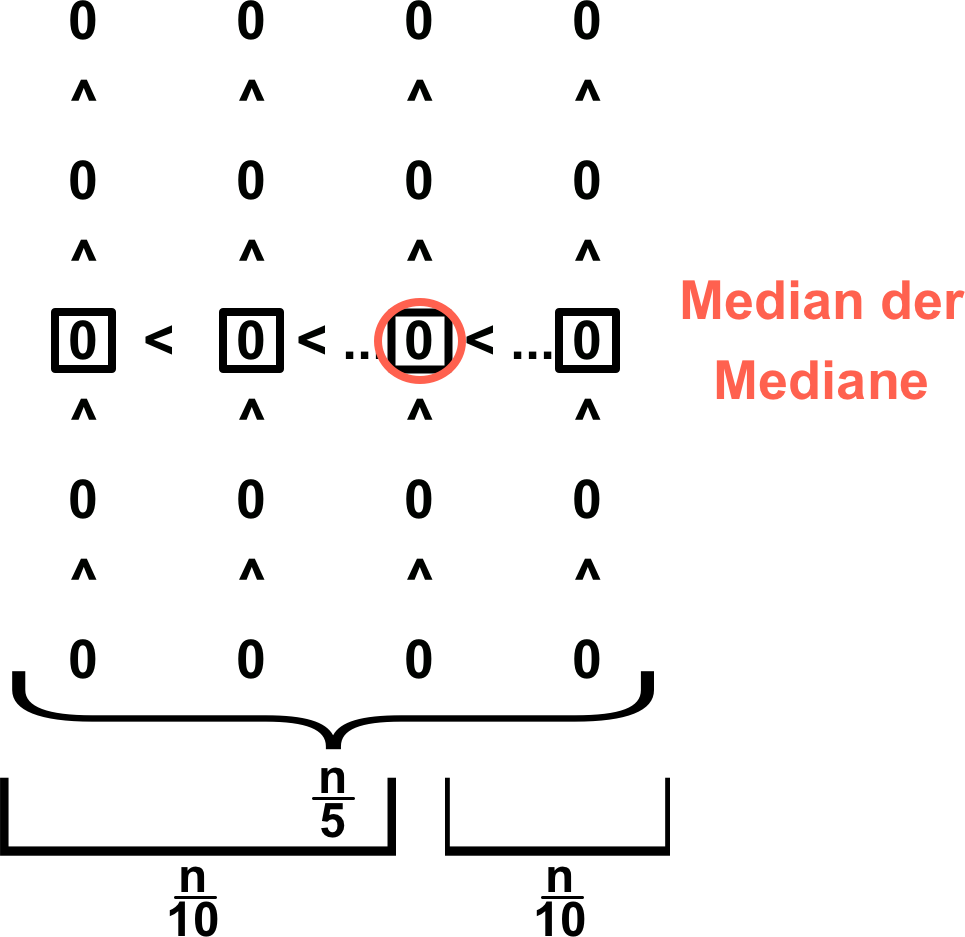
\includegraphics[width=\linewidth]{8/Grafik/img1.png}
\caption{}
\end{wrapfigure}

\vspace{30pt}
\paragraph{Wortlaut}
Teile die n Elemente in 5-er Gruppen. Bestimme innerhalb jeder Gruppe den Median. Bestimme nun den Median der Mediane.
\vspace{50pt}


\newpage


\subsection{Deterministische Variante für K-Select}

\subsection{Laufzeitanalyse für den worst-case}


\section{Untere Schranke für vergleichsbasierte Sortierverfahren}